% =====================================================================
%  IN6049 --- Forecasting and Regression Analysis
%  Week 3: Simultaneous Inferences and Other Topics --- Tips dataset
%
%  Built from template/slides-template.tex (Boadilla + seahorse, 16:9).
%  Title slide + 4 content slides.  Numbers come from Assigment_2.ipynb
%  (Lecture 3 section); figures are the notebook's own PNGs.
%
%  Compiles on Overleaf with the default pdfLaTeX engine.
%  Upload alongside: fig_ellipse.png , fig_wh.png , fig_bands.png , fig_origin.png
% =====================================================================
\documentclass[aspectratio=169,11pt]{beamer}

\usetheme{Boadilla}
\usecolortheme{seahorse}
\setbeamertemplate{navigation symbols}{}

\usepackage[utf8]{inputenc}
\usepackage[T1]{fontenc}
\usepackage{booktabs}
\usepackage{amsmath}
\usepackage{graphicx}
\usepackage{url}

\newcommand{\key}[1]{\textbf{\structure{#1}}}

% ---------------------------------------------------------------------
\title[Simultaneous inferences]{Simultaneous Inferences --- Restaurant Tips}
\subtitle{From one interval to a family of statements}
\author[Jie Dong, Elivier Reyes]{Jie Dong, Elivier Reyes}
\date[IN6049]{}

\begin{document}

% ===================== TITLE ========================================
\begin{frame}
  \titlepage
  \vspace{-1.2em}
  \begin{center}
    \small\urlstyle{same}\url{https://github.com/HelloJJJie/Assignment-Forecast-and-Analysis-of-Regression.git}

    \vspace{1.2em}
    A dataset of $n=244$ restaurant bills --- how sure can we be about
    \emph{several} statements at the same time?
  \end{center}
\end{frame}

% ===================== 1. WHY SIMULTANEOUS ==========================
\begin{frame}{1. Why simultaneous inference? Joint intervals for $\beta_0,\beta_1$}
  \begin{columns}[T]
  \begin{column}{0.52\textwidth}
    \small
    \key{Data.} \texttt{tips.csv}, $X=$ total bill, $Y=$ tip (USD);
    $\hat Y=0.920+0.105X$.

    \vspace{0.3em}
    \key{Problem.} A $95\%$ interval is right \emph{one statement at a time}.
    For $g$ statements, $P(\text{all correct})\ge 1-g\alpha$ (Bonferroni), so each
    interval needs level $1-\alpha/g$.

    \vspace{0.4em}
    {\scriptsize\textit{Share of runs in which the interval(s) cover the truth:}

    \vspace{0.1em}
    \begin{tabular}{@{}lrrrr@{}}
      \toprule
      Intervals & mult. & $\beta_0$ & $\beta_1$ & \textbf{both} \\
      \midrule
      two separate $95\%$     & $1.970$ & $.945$ & $.947$ & $\mathbf{.927}$ \\
      Bonferroni, fam.\ $95\%$ & $2.255$ & $.973$ & $.975$ & $\mathbf{.962}$ \\
      \bottomrule
    \end{tabular}}

    \vspace{0.2em}
    {\scriptsize Simulated: $5000$ synthetic data sets drawn from the fitted
     model (normal errors, same $X$); Monte-Carlo s.e.\ $\approx0.003$.\par}

    \vspace{0.3em}
    \small
    Separate intervals fall \emph{below} $95\%$ jointly; Bonferroni guarantees
    at least $95\%$ and here lands at $96.2\%$ --- conservative, but safe.
  \end{column}
  \begin{column}{0.48\textwidth}
    \centering
    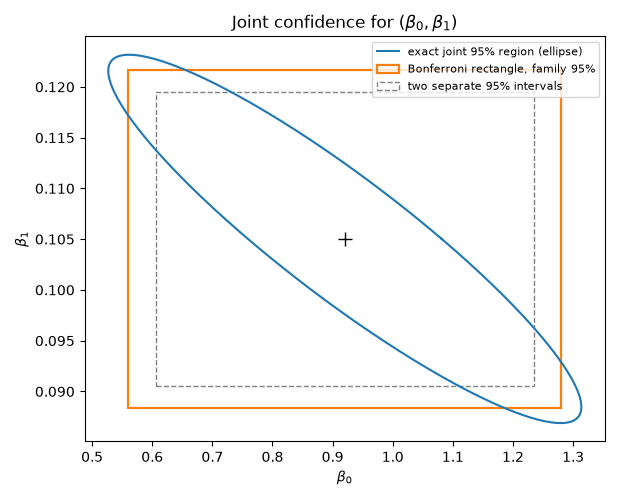
\includegraphics[width=0.78\linewidth]{fig_ellipse.png}

    \vspace{0.2em}
    {\scriptsize
    \begin{tabular}{@{}lcc@{}}
      \toprule
       & single $95\%$ & family $95\%$ \\
      \midrule
      $\beta_0$ & $[0.606,\,1.235]$ & $[0.560,\,1.281]$ \\
      $\beta_1$ & $[0.0905,\,0.1195]$ & $[0.0884,\,0.1216]$ \\
      \bottomrule
    \end{tabular}}

    \vspace{0.2em}
    {\scriptsize The exact joint region is a tilted ellipse, since
     $\mathrm{corr}(b_0,b_1)=-0.91$.\par}
  \end{column}
  \end{columns}
\end{frame}

% ===================== 2. MEAN RESPONSE =============================
\begin{frame}{2. Mean response: one band for the whole line}
  \begin{columns}[T]
  \begin{column}{0.50\textwidth}
    \small
    Estimate $E\{Y_h\}$ at several $X_h$ at once, $\hat Y_h\pm(\text{mult})\,s\{\hat Y_h\}$:
    \begin{itemize}
      \item \key{Working--Hotelling:} $W^2=2F(1-\alpha;2,n-2)$, so $W=2.463$.
            Holds for \emph{all} $X_h$ --- the whole line --- and does not
            depend on $g$.
      \item \key{Bonferroni:} $B=t(1-\alpha/2g;\,n-2)$, only for the $g$
            stated levels, and it grows with $g$.
      \item \key{Use the smaller.} The band is $W/t=1.25\times$ the pointwise
            interval ($t=1.970$), at every $X$.
    \end{itemize}

    \vspace{0.2em}
    {\scriptsize
    \begin{tabular}{@{}l@{\hskip 0.8em}rrrrr@{\hskip 1.2em}r@{}}
      \toprule
      $g$ & $2$ & $3$ & $4$ & $5$ & $10$ & $W$ \\
      \midrule
      $B$ & $2.255$ & $2.411$ & $2.517$ & $2.596$ & $2.833$ & $2.463$ \\
      \bottomrule
    \end{tabular}}

    \vspace{0.2em}
    {\small Bonferroni wins only for $g\le3$ here.\par}
  \end{column}
  \begin{column}{0.50\textwidth}
    \centering
    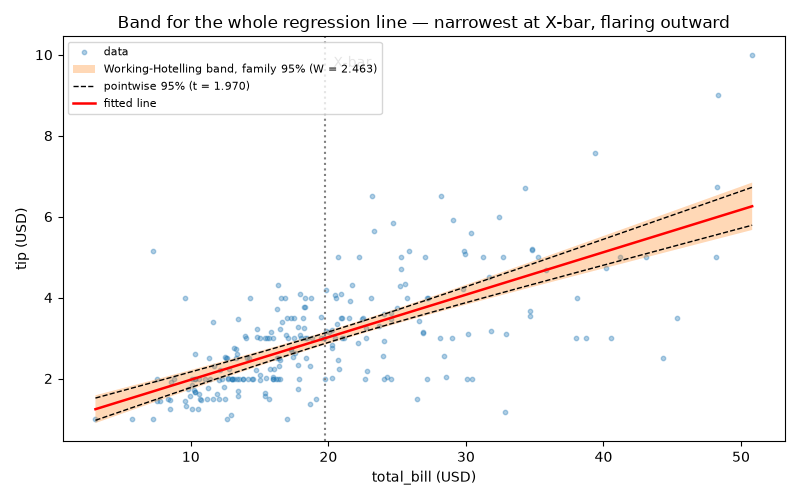
\includegraphics[width=0.84\linewidth]{fig_wh.png}

    \vspace{0.3em}
    {\scriptsize
    \begin{tabular}{@{}rrcc@{}}
      \toprule
      $X_h$ & $\hat Y_h$ & W--H, $g=3$ & Bonferroni, $g=3$ \\
      \midrule
      $10$ & $1.971$ & $[1.731,\,2.210]$ & $[1.736,\,2.205]$ \\
      $20$ & $3.021$ & $[2.860,\,3.182]$ & $[2.863,\,3.179]$ \\
      $30$ & $4.071$ & $[3.825,\,4.317]$ & $[3.831,\,4.311]$ \\
      \bottomrule
    \end{tabular}}
  \end{column}
  \end{columns}
\end{frame}

% ===================== 3. PREDICTION ================================
\begin{frame}{3. Predicting new tips: the prediction band}
  \begin{columns}[T]
  \begin{column}{0.50\textwidth}
    \small
    For $g$ new observations,
    $s^2\{pred\}=MSE\big[\,\mathbf{1}+\tfrac1n+\tfrac{(X_h-\bar X)^2}{\sum(X_i-\bar X)^2}\big]$:
    the extra $1$ is the new tip's own scatter.
    \begin{itemize}
      \item \key{Scheff\'e} $S=2.815$ vs.\ \key{Bonferroni} $B=2.411$
            ($g=3$): use Bonferroni.
      \item At $\bar X$ the prediction band is about $15\times$ wider than the
            Working--Hotelling band.
      \item \key{Intervals can leave the possible range:} at $X_h=10$ the lower
            limit is $-0.51$, but a tip cannot be negative.
      \item \key{Constant width, growing scatter:} the pointwise $95\%$
            interval holds $97.5\%$ of tips in the lowest third of bills but only
            $81.9\%$ in the highest ($93.0\%$ overall).
    \end{itemize}
  \end{column}
  \begin{column}{0.50\textwidth}
    \centering
    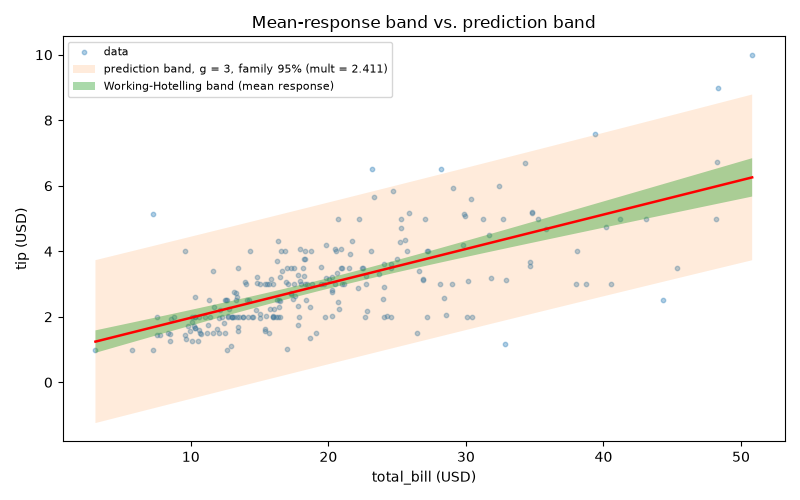
\includegraphics[width=0.84\linewidth]{fig_bands.png}

    \vspace{0.3em}
    {\scriptsize
    \begin{tabular}{@{}rrcc@{}}
      \toprule
      $X_h$ & $\hat Y_h$ & $s\{pred\}$ & family $95\%$ PI \\
      \midrule
      $10$ & $1.971$ & $1.027$ & $[-0.505,\,4.446]$ \\
      $20$ & $3.021$ & $1.024$ & $[\,0.552,\,5.490]$ \\
      $30$ & $4.071$ & $1.027$ & $[\,1.595,\,6.547]$ \\
      \bottomrule
    \end{tabular}}
  \end{column}
  \end{columns}
\end{frame}

% ===================== 4. OTHER TOPICS ==============================
\begin{frame}{4. Other topics and takeaway}
  \begin{columns}[T]
  \begin{column}{0.44\textwidth}
    \centering
    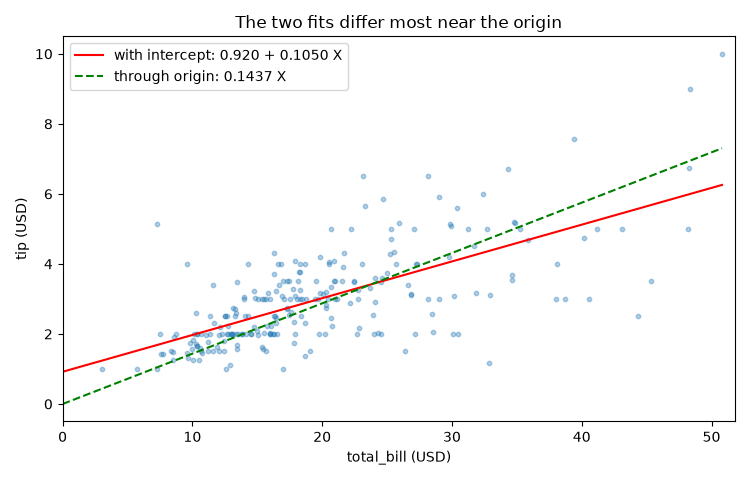
\includegraphics[width=0.78\linewidth]{fig_origin.png}

    \vspace{0.2em}
    {\scriptsize
    \begin{tabular}{@{}lrr@{}}
      \toprule
       & Intercept & Origin \\
      \midrule
      $b_1$             & $0.105$  & $0.144$ \\
      $s\{b_1\}$        & $0.0074$ & $0.0032$ \\
      $MSE$ (df)        & $1.045$ ($242$) & $1.183$ ($243$) \\
      ``$R^2$''         & $0.457$  & $0.892^{*}$ \\
      \bottomrule
    \end{tabular}}

    \vspace{0.1em}
    {\tiny$^{*}$uncentred; not comparable with $0.457$.}
  \end{column}
  \begin{column}{0.54\textwidth}
    \small
    \begin{itemize}
      \item \key{Through the origin} is defensible on theory (zero bill, zero
            tip), but the data object: $t^{*}=5.76$ for $\beta_0=0$.
      \item \key{Inverse prediction:} a $\$5$ tip gives
            $\hat X=38.85$, interval $[19.5,\,58.2]$ --- wider than the observed
            bills ($3$--$51$); with $r=0.676$ a tip pins the bill down poorly.
      \item \key{Design:} $s\{b_1\}$ would be $0.0316$ with only the middle half
            of the bills (observed: $0.0074$); $s\{\hat Y_h\}$ at $X_h=45$ is
            $3\times$ its value at $\bar X$.
    \end{itemize}

    \vspace{0.3em}
    \key{Takeaway.} Several statements at once cost a wider interval: choose the
    procedure by $g$ and by what is being claimed. Intervals for \emph{new}
    observations also lean on constant variance and normality, which the earlier
    diagnostics put in doubt.
  \end{column}
  \end{columns}
\end{frame}

\end{document}
